\documentclass[11pt]{article}

\usepackage[T1]{fontenc}
\usepackage[polish]{babel}
\usepackage[utf8]{inputenc}
\usepackage{lmodern}
\selectlanguage{polish}

\usepackage{graphics}
\usepackage{graphicx}

\author{Michał Bobowski, Marcin Cieślikowski}
\date{2014-01-16}
\title{Narzędzie do analizy statystycznej słów i bigramów.}

\begin{document}
  \maketitle

\section{Wstęp}
Niniejszy dokument stanowi podsumowanie projektu z przedmiotu WEDT.
Zawiera opis interfejsu użytkownika i logiki programu oraz przedstawienie struktury kodu źródłowego.

\section{Koncepcja programu}
Program ma za zadanie obliczyć statystyki słów i bigramów z jednego lub wielu plików wejściowych.
Obsługiwane powinny być najbardziej popularne formaty plików w tym pliki MS Word.
Wyniki obliczeń powinny być przechowywane na dysku w rozsądnym formacie i możliwe do wykorzystania w przyszłości.

Program powinien zawierać prosty graficzny interfejs użytkownika.
Jego zadaniem jest pobranie parametrów obliczeń oraz wyświetlenie wyników symulacji.
Możliwa powinna być również filtracja wyświetlanych danych danych.

\section{Przypadki użycia}
\subsection{Przeprowadzenie obliczeń}
Podstawowym zadaniem programu jest przeprowadzenie obliczeń i wyświetlenie ich na ekranie.
Scenariusz tworzą następujące zdarzenia:
\begin{enumerate}
 \item Użytkownik wybiera parametry.
 \item System przeprowadza obliczenia.
 \item System zapisuje wyniki do pliku.
 \item System wyświetla wyniki na ekranie.
\end{enumerate}

\subsection{Wczytanie wyników}
\begin{enumerate}
 \item Użytkownik wybiera ścieżkę do pliku z zapisanymi wynikami.
 \item System wyświetla wyniki na ekranie.
\end{enumerate}

\subsection{Filtracja}
Operacja filtracji staje się dostępna dopiero po wykonaniu któregoś z wcześniejszych przypadków użycia.
\begin{enumerate}
 \item Użytkownik wybiera jedną z tabel wynikowych.
 \item Użytkownik wypełnia filtry.
 \item System wyświetla przefiltrowane wyniki na ekranie.
\end{enumerate}

\section{Specyfikacja szczegółowa}
W tej części doprecyzowane zostały wymagania dotyczące danych wejściowych i wyjściowych.
\subsection{Parametry wejściowe}
Przed przeprowadzeniem obliczeń użytkownik może zdefiniować następujące parametry:
\begin{enumerate}
 \item Ścieżka do pliku wejściowego lub katalogu zawierającego wiele plików wejściowych.
 \item Typ bigramu: obliczany dla kolejnych słów lub wszystkich słów w tekście.
 \item Części mowy dla słów z bigramu.
 \item Nazwa pliku wyjściowego.
\end{enumerate}

\subsection{Prezentacja danych}
Statystyki słów/bigramów są liczone i prezentowane dwa razy - dla słów z odmianą oraz dla formy podstawowej.
Statystyki dla słów:
\begin{enumerate}
 \item Liczba wystąpień w zbiorze.
 \item Liczba zdań w których wystąpiło słowo.
 \item Liczba dokumentów w których wystąpiło słowo.
 \item Procent dokumentów w których wystąpiło słowo.
 \item Miara tf-idf.
\end{enumerate}

Statystyki dla bigramów:
\begin{enumerate}
 \item Liczba wystąpień w zbiorze.
 \item Liczba zdań w którtch wystąpił bigram.
 \item Liczba dokumentów w których wystąpił bigram.
 \item Procent dokumentów w których wystąpił bigram.
 \item Miara tf-idf.
 \item Prawdopodobieństwo słowa 1.
 \item Prawdopodobieństwo słowa 2.
 \item Prawdopodobieństwo bigramu złożonego ze słów 1 i 2.
\end{enumerate}

\subsection{Format danych wyjściowych}
Dane wyjściowe są zapisywane do pliku bazy danych sqlite.
Baza danych zawiera 8 nastepujących tabel:
\begin{enumerate}
 \item Tabela words zawiera statystyki słow. Tabela ta zawiera następujące pola:
  \begin{enumerate}
    \item word - Nazwa słowa.
    \item count - Liczba wystąpień słowa w korpusie.
    \item numberOfSentences - Liczba zdań zawierających słowo.
    \item numberOfDocuments - Liczba dokumentów zawierających słowo.
    \item percentOfDocuments - Procent dokumentów zawierających słowo.
  \end{enumerate}
  \item Tabela Lemmas zawiera statystyki dla słów w formie podstawowej. Pola tej tabeli są identyczne, jak w tabeli words.
  \item Tabela WordTFIDF - Zawiera wskaźnik TF-IDF. W~tej tabeli znajdują się następujące pola:
  \begin{enumerate}
    \item word - Słowo, dla którego obliczany jest wskaźnik TF-IDF.
    \item  document - Nazwa dokumentu, dla którego oblicznay jest wskaźnik TF-IDF.
    \item TFIDF - Wartość wskaźnika TFIDF
  \end{enumerate}
  \item Tabela bigrams zawiera statystyki bigramów. Tabela ta zawiera następujące pola:
  \begin{enumerate}
     \item word1 - Pierwsze słowo w bigramie.
     \item word2 - Drugie słowo w bigramie.
     \item count - Liczba wystąpień bigramu w korpusie.
     \item numberOfSentences  - Liczba zdań zawierające bigram.
     \item numberOfDocuments - Liczba dokumentów zawierających bigram.
     \item percentOfDocuments  - Procent dokumentów zawierających bigram.
     \item percentOfSentence  -  Procent zdań zawierająch bigram.
     \item percentOfSentencew1 - Procent zdań zawierająch pierwsze zdanie.
     \item percentOfSentencew2 - Procent zdań zawierająch drugie zdanie.
  \end{enumerate}
  \item Tabela bigramsLemma zawiera statystyki bgramów w formie podstawowej. Pola tabeli są takie same, jak w tabeli bigrams.
  \item Tabela bigramsTFIDF zawiera wskaźnik TF-IDF dla bigramów. Tabela zawiera następujące pola:
  \begin{enumerate}
     \item word1 - Pierwsze słowo w bigramie.
     \item word2 - Drugie słowo w bigramie.
     \item  TFIDF - Wartość wskaźnika TFIDF
  \end{enumerate}
  \item Tabela bigramsLemmaTFIDF zawiera wskaźnik TF-IDF dla bigramów w formie podstawowej.
  Pola tabeli pokrywaja się z polami tabel bigramsTFIDF
\end{enumerate}
\section{Wybór narzędzi i technologii}
Program został zrealizowany w języku Java.
Kod tworzyliśmy przy użyciu środowiska Eclipse oraz częściowo Netbeans (edytor interfejsu użytkownika).
Do kontroli kodu wykorzystaliśmy system Git.

Do oznaczenia części mowy wykorzystaliśmy bibliotekę Gate.
Korzysta ona wewnętrznie z biblioteki TIKA, dzięki czemu uzyskaliśmy wsparcie dla wielu formatów tekstowych m. in. txt, html, odt i doc.

\section{Opis kodu źródłowego}

\section{Algorytmy}
Program dla podanych dokumentów uruchamia funkcje bibliotęki GATE, które dzielą tekst na słowa, zdania. Dodatkowo dla słów są określanę części mowy i formy podstawowe słów.
Dane zwróconę przez GATE są przetwarzane do formy przedstwionej na rysunku 1.
\begin{figure}
  \begin{center}
    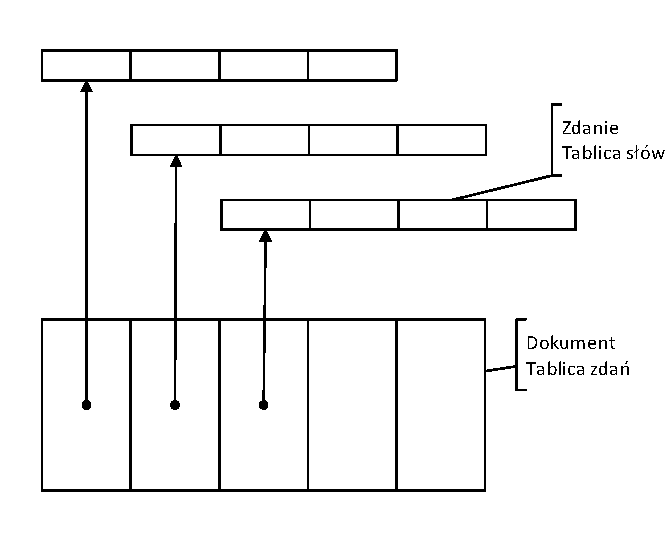
\includegraphics{Struktura danych.pdf}
    \caption{Struktura danych}
  \end{center}
\end{figure}
Program przetwarza po kolei termy (słowa i bigramy) w~zdaniach. Podczas przetwarzania termów program zlicza statystyki termów.
 


\end{document}